% =====================================================================
% CENG391 term project report: one template for both reports.
%
%   Progress Report (20 November 2026): keep \finalfalse   (default)
%   Final Report    (4 January 2027):   change to \finaltrue
%
% Build:  latexmk -pdf main.tex        (or upload this folder to Overleaf)
% The Progress Report PDF must be named after the group id, e.g. G11.pdf.
% Red [TODO: ...] notes mark everything that still has to be written.
% The sections live in sections/ so that several people can write at once.
% See README.md in this folder.
% =====================================================================
\documentclass[11pt,a4paper]{article}

\newif\iffinal
\finalfalse

\usepackage[utf8]{inputenc}
\usepackage[T1]{fontenc}
\usepackage{lmodern}
\usepackage[a4paper,margin=2.5cm]{geometry}
\usepackage{amsmath,amssymb}
\usepackage{graphicx}
\usepackage{booktabs}
\usepackage{array}
\usepackage{enumitem}
\usepackage{xcolor}
\usepackage{tikz}
\usetikzlibrary{positioning}
\usepackage{pgfgantt}
\usepackage[colorlinks=true,linkcolor=black,citecolor=black,urlcolor=blue]{hyperref}

% ---- things to fill in once --------------------------------------------
\newcommand{\groupid}{G\textbf{??}}
\newcommand{\projecttitle}{Real-Time Hand Gesture Interface}
\newcommand{\members}{\textcolor{red}{[TODO: full names and student numbers]}}

% ---- helpers ---------------------------------------------------------------
\newcommand{\todo}[1]{\textcolor{red}{[TODO: #1]}}
\newcommand{\vect}[1]{\mathbf{#1}}

\title{\projecttitle\\[2pt]\large CENG391 Term Project --- \iffinal Final\else Progress\fi\ Report}
\author{Group \groupid\\ \members}
\date{\iffinal 4 January 2027\else 20 November 2026\fi}

\begin{document}
\maketitle

\iffinal
\begin{abstract}
\todo{Single paragraph, at most about 250 words. Written last.}
\end{abstract}
\fi

\section{Introduction}

% Progress Report: 1.1, 1.2 and 1.4 (about half a page to one page in total).
% Final Report: all subsections.

\subsection{Motivation and Application Context}
% WRITE: why touchless gesture control is useful, with two or three concrete use cases.
\todo{two or three concrete use cases}

\subsection{Problem Statement}
% WRITE: what the system must infer from camera images and why this is hard:
% lighting, background, camera distance, differences between users, and the difference
% between an intentional gesture and an incidental movement (the ``Midas touch'' problem).
\todo{problem statement}

\iffinal
\subsection{Aim and Objectives}
% WRITE: one sentence for the aim, then a list of objectives.
\todo{aim and objectives}
\fi

\subsection{Proposed Approach}
% WRITE: the pipeline in short, from camera input to the recognised gesture:
% camera -> hand landmarks (MediaPipe) -> smoothing -> normalisation -> segmentation
% -> static and dynamic classification -> false-trigger prevention.
% Say clearly that the hand model is pretrained and that our contribution is what is built
% on its output and how it is evaluated.
\todo{approach in one paragraph; refer to Figure~\ref{fig:pipeline}}

\iffinal
\subsection{Contributions}
% WRITE: three or four points.
\todo{contributions}

\subsection{Report Organization}
% WRITE: one sentence per remaining section.
\todo{report organisation}
\fi

\section{Related Work}

% Progress Report: one short paragraph for 2.1, 2.3, 2.4 and 2.5, one sentence for 2.2 (1 to 1.5 pages).
% Each subsection must justify one choice of the methodology. Write it as an argument, not as a list.
% Candidate works are in literature.bib; every entry there is UNVERIFIED and must be checked
% against the original paper before it is cited.

\subsection{Hand Detection and Landmark Estimation}
% JUSTIFIES: why MediaPipe Hands.
% COVER: classical methods (skin colour, contour, hand-crafted features) and their sensitivity to
% lighting and background; MediaPipe Hands, a palm detector followed by a 21-landmark regression model.
% CITE (after checking): zhang2020mediapipe
\todo{2.1}

\subsection{Gesture Datasets and Benchmarks}
% JUSTIFIES: why we record our own data.
% COVER: size, classes, static or dynamic content and fit for device control of public datasets;
% none of them is recorded under controlled, labelled lighting, background and distance conditions.
% CITE (after checking): kapitanov2022hagrid, materzynska2019jester, benitezgarcia2020ipn
\todo{2.2 (Progress Report: one sentence)}

\subsection{Static and Dynamic Gesture Recognition}
% JUSTIFIES: why landmark-based features and small models.
% COVER: landmark-based versus video-based recognition, classical versus learned classifiers.
% CITE (after checking): molchanov2016online
\todo{2.3}

\subsection{Continuous Recognition and False-Trigger Prevention}
% JUSTIFIES: why segmentation with hysteresis, a hold time and a cooldown.
% COVER: how existing work finds the start and end of a gesture, rejects movements that are not
% gestures, and measures false positives and latency.
% CITE (after checking): alon2009unified, jacob1990what
\todo{2.4}

\subsection{Temporal Smoothing}
% JUSTIFIES: why the 1-euro filter.
% COVER: noisy landmark streams, the jitter versus lag trade-off.
% CITE (after checking): casiez2012oneeuro
\todo{2.5}

\iffinal
\subsection{Comparison and Positioning}
% WRITE: a table of the cited works and one sentence on how this project differs, for example:
% existing work mostly reports accuracy under one condition, while this project evaluates
% robustness across users, backgrounds, lighting and distance, and measures false-trigger
% rate and latency explicitly.
\todo{comparison table and positioning}
\fi

\section{Dataset and Problem Definition}

% Progress Report: 3.1 and 3.2 in full, 3.3 to 3.6 as the PLANNED protocol (one short paragraph each
% or less). 3.7 and 3.8 are Final Report only.

\subsection{Task Definition}
% WRITE: the input is a continuous RGB stream from a single ordinary webcam; the output is the
% recognised gesture (or ``no gesture''). Three tasks: static classification, dynamic
% classification, temporal segmentation. Name the difficulties that will be evaluated
% (lighting, background, camera distance, users, intentional versus incidental movement) and the
% constraints (real time, ordinary webcam, no extra hardware).
\todo{task definition}

\subsection{Gesture Set}
% The gesture set below is DECIDED. Commands are not defined yet: the system only recognises the
% gestures for now. The label names are the ones in dataset_config.py.
\begin{table}[h]
\centering
\begin{tabular}{@{}lll p{6.2cm}@{}}
\toprule
Label & Type & Hand & Description \\
\midrule
\texttt{fist}        & static  & closed hand & held still \\
\texttt{open\_palm}  & static  & open hand & fingers extended, held still \\
\texttt{thumb\_up}   & static  & fist & thumb pointing up, held still \\
\texttt{thumb\_down} & static  & fist & thumb pointing down, held still \\
\texttt{point}       & static  & index finger & index finger extended, other fingers closed \\
\texttt{swipe\_left}  & dynamic & open palm & out-and-back movement; first stroke towards the user's left \\
\texttt{swipe\_right} & dynamic & open palm & out-and-back movement; first stroke towards the user's right \\
\texttt{no\_gesture}  & both    & any & negative class: poses and movements that are not one of the gestures \\
\bottomrule
\end{tabular}
\caption{Gesture set. \todo{decide whether to add the commands (target device) before the Final Report}}
\label{tab:gestures}
\end{table}
% WRITE: one sentence per gesture on why it was chosen (visually distinct, easy to perform, not
% confusable). Explain that the open palm is used both as a static gesture and for swipes, and
% that the two are told apart by movement (see Section on segmentation).

\subsection{Data Collection Protocol}
% PLANNED protocol (Progress Report).
% FACTS from the project, check before use:
%  - camera 640 x 480, about 20 frames per second while recording;
%  - only the 21 hand landmarks are stored, not the images; clips are labelled with user,
%    gesture, background, lighting and distance;
%  - static clips: 2 seconds, hand held completely still; swipe and no_gesture clips: 3 seconds;
%  - swipe: wait about half a second after the countdown, make the out-and-back movement once at a
%    steady speed with a large amplitude (about one hand size or more), then keep the hand still;
%  - participants give consent; raw video is not kept.
\todo{protocol}

\subsection{Participants and Recording Conditions}
% PLANNED (Progress Report). Fill in the real numbers.
\begin{table}[h]
\centering
\begin{tabular}{@{}lll@{}}
\toprule
Factor & Levels & Planned \\
\midrule
Users & \todo{how many} & \todo{} \\
Background & plain, cluttered & \todo{} \\
Lighting & bright, dim & \todo{} \\
Camera distance & near, far & \todo{} \\
\bottomrule
\end{tabular}
\caption{Recording conditions.}
\end{table}

\subsection{Dataset Statistics}
% Numbers come from validate_dataset.py (clips per user, gesture and condition).
% Progress Report: planned numbers, or the pilot numbers clearly marked as pilot.
\todo{statistics table}

\subsection{Train, Validation and Test Split}
% WRITE: the split is by PERSON, never by frame or clip, because frames of one clip are nearly
% identical and would leak into the test set. Test users are not used while choosing thresholds or
% models; they are used once, at the end. With few users, leave-one-user-out cross-validation.
\todo{split}

\iffinal
\subsection{Preprocessing and Augmentation}
% WRITE: smoothing, normalisation, stable-frame selection; any augmentation (for example random
% rotation of the training frames).
\todo{preprocessing and augmentation}

\subsection{Data Limitations}
% WRITE: known biases and gaps (number of users, one camera, one environment, ...).
\todo{limitations}
\fi

\section{Methodology}

% Progress Report (requirement 2, ``Methodology and Implementation''): this is the main section.
% One paragraph and the needed formula per subsection, plus the implementation work completed so far
% (subsection 4.11). Use the same terms everywhere: landmark, normalisation, segmentation, hold time,
% cooldown, no-gesture class. TEAM_BRIEF_methodology.md (repository root) has the reasoning behind each stage.

\subsection{System Overview}
% WRITE: a short description of each stage. The pipeline runs smoothing BEFORE normalisation
% (smoothing works on the raw landmarks), although Section 4.3 is written before 4.4.
% Calibration is a start-up step that sets parameters of later stages, not a stage of the
% per-frame chain. Mention where the delay is measured (experiment E9).
\begin{figure}[H]
\centering
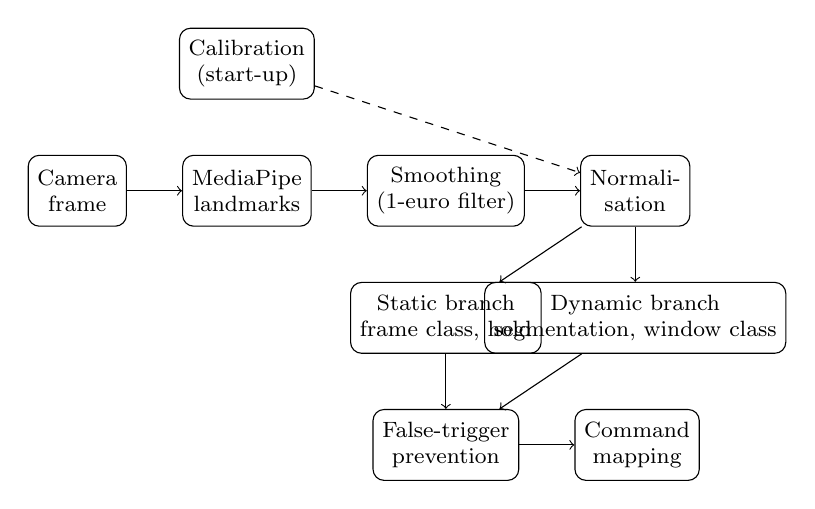
\begin{tikzpicture}[node distance=7mm and 7mm,
  box/.style={draw, rounded corners, align=center, minimum height=9mm, font=\footnotesize}]
  \node[box] (cam) {Camera\\frame};
  \node[box, right=of cam] (lm) {MediaPipe\\landmarks};
  \node[box, right=of lm] (sm) {Smoothing\\(1-euro filter)};
  \node[box, right=of sm] (nm) {Normali-\\sation};
  \node[box, below=of sm] (st) {Static branch\\frame class, hold};
  \node[box, below=of nm] (dy) {Dynamic branch\\segmentation, window class};
  \node[box, below=of st] (ft) {False-trigger\\prevention};
  \node[box, right=of ft] (cmd) {Command\\mapping};
  \node[box, above=of lm] (cal) {Calibration\\(start-up)};
  \draw[->] (cam) -- (lm);
  \draw[->] (lm) -- (sm);
  \draw[->] (sm) -- (nm);
  \draw[->] (nm) -- (st);
  \draw[->] (nm) -- (dy);
  \draw[->] (st) -- (ft);
  \draw[->] (dy) -- (ft);
  \draw[->] (ft) -- (cmd);
  \draw[->, dashed] (cal) -- (nm);
\end{tikzpicture}
\caption{Processing pipeline. Calibration (dashed) sets the hand scale and the thresholds of later
stages. \todo{redraw if needed; add the delay measurement points}}
\label{fig:pipeline}
\end{figure}

\subsection{Hand Detection and Landmark Extraction}
% WRITE: MediaPipe Hands (palm detector, then a landmark model); the output is 21 points
% (x, y, z) per hand; settings (one hand, detection and tracking confidence); a frame without a
% hand counts as ``no gesture''. State openly that the model is pretrained and not ours.
\todo{4.2}

\subsection{Landmark Normalisation and Features}
% WRITE: why raw coordinates depend on position and distance, and the two steps.
% x and y are first converted to pixel units (MediaPipe divides them by the image width and height,
% so equal steps are different lengths on a 4:3 camera); rotation is deliberately NOT removed.
\begin{equation}
  \hat{\vect{q}}_i = \frac{\vect{p}_i - \vect{p}_0}{s}, \qquad
  s = \lVert \vect{p}_9 - \vect{p}_0 \rVert , \quad i = 0, \dots, 20
\end{equation}
% p_0 is the wrist, p_9 the base of the middle finger, s the hand size measured in the image plane.
\todo{4.3: explain the equation; feature vector (63 numbers) and any derived features}

\subsection{Temporal Smoothing}
% WRITE: the jitter versus lag trade-off and the 1-euro filter (Casiez et al.), applied per
% coordinate to the raw landmarks. The filter is causal, so it works on the live stream.
\begin{align}
  \hat{\dot{x}}_t &= \alpha(d_c)\,\dot{x}_t + \bigl(1 - \alpha(d_c)\bigr)\,\hat{\dot{x}}_{t-1}, \\
  f_c &= f_{c,\min} + \beta\,\lvert \hat{\dot{x}}_t \rvert, \\
  \alpha(f) &= \frac{1}{1 + \tau / T_e}, \quad \tau = \frac{1}{2\pi f}, \\
  \hat{x}_t &= \alpha(f_c)\,x_t + \bigl(1 - \alpha(f_c)\bigr)\,\hat{x}_{t-1},
\end{align}
% with T_e the time between two frames. Tuning order: beta = 0 and f_cmin against jitter on a still
% hand, then beta against the lag in fast movements.
% PROVISIONAL values from the pilot clips of one hand: f_cmin = 0.5 Hz, beta = 0.02, d_c = 1 Hz.
\todo{4.4: parameter table with the final values and how they were chosen}

\subsection{Gesture Segmentation}
% WRITE: static gestures: the same class for several consecutive frames while the hand is nearly
% still (hold). Dynamic gestures: speed of the palm centre against two thresholds with hysteresis;
% the window runs from the onset of the outward stroke until the hand is still again.
% Segmentation decides ``is this a gesture candidate?''; Section 4.9 decides ``should it become a
% command?''. Do not mix the two.
\begin{equation}
  \vect{c}_t = \frac{1}{5}\sum_{i \in \{0, 5, 9, 13, 17\}} \vect{p}_i(t), \qquad
  v_t = \frac{\lVert \vect{c}_t - \vect{c}_{t-1} \rVert}{s\,\Delta t}
\end{equation}
% The palm centre c_t is used instead of the wrist because in the pilot the wrist moved only about
% half as far (the hand pivots at the wrist). Onset when v_t > tau_on, end when v_t < tau_off
% (tau_on > tau_off), with a minimum duration.
% Open palm is both a static gesture and the hand shape of the swipes: the static branch is
% suppressed while v_t is above the threshold, needs a hold time, and is blocked for about a second
% after a swipe cycle.
\todo{4.5 (Progress Report: the static part exists as the stable-frame selection of the data loader; the swipe segmentation is planned)}

\subsection{Static Gesture Classification}
% WRITE: input (normalised landmarks of one frame), the rule-based baseline and the learned model
% (SVM with RBF kernel on standardised inputs), training data (stable frames only), how results are
% measured (per clip or per user, never per frame).
% WARNING from the pilot: the first classifier learned the TILT of the hand, because only the thumb-up
% clips were tilted in the training data. Say how this is handled (varied orientations in the
% recordings, rotation-independent features, rotation augmentation).
\todo{4.6}

\subsection{Dynamic Gesture Classification}
% WRITE: window of the out-and-back movement resampled to a fixed length, expressed relative to its
% starting position; rule-based baseline (direction of the first stroke) versus a small learned model.
\todo{4.7 (Progress Report: planned)}

\subsection{User Calibration}
% WRITE: what is measured at start-up (hand size, typical speed) and which parameters it adjusts
% (scale, segmentation thresholds, confidence threshold).
\todo{4.8 (Progress Report: planned)}

\subsection{False-Trigger Prevention}
% WRITE: confidence threshold, stability check, the no-gesture class, cooldown after a swipe.
% DECIDED (TEAM_BRIEF D.4 items 10 and 11): NO activation gesture, a command starts as soon as its
% gesture is recognised (like pressing a phone's volume key); while a static gesture is held its
% command repeats step by step until the gesture is released. Say why no clutch is used and what
% protects against accidental commands instead.
\todo{4.9 (Progress Report: planned)}

\subsection{Command Mapping and Device Control}
% Commands and target device are not decided yet; say so, or leave the subsection out of the Progress Report.
\todo{4.10}

\subsection{Implementation Details}
% FACTS: Python 3.10; MediaPipe 1.2.3 (Tasks API, HandLandmarker); OpenCV; NumPy; scikit-learn 1.7.2.
% See README.md in the repository root for the exact steps to run the code.
\todo{4.11: language, libraries and versions, hardware, how to run}

\iffinal\else
\subsubsection*{Implementation Progress}
% Progress Report requirement 2: ``describe the implementation work completed so far''.
% Keep completed work and planned work clearly apart. Update this table on the day of submission.
\begin{table}[H]
\centering
\begin{tabular}{@{}lp{6.8cm}c@{}}
\toprule
Component & Status & Section \\
\midrule
Landmark extraction (MediaPipe) & implemented in the recording tool & 4.2 \\
Recording, viewing and validation tools & done & 3 \\
Normalisation & done and tested & 4.3 \\
Temporal smoothing (1-euro filter) & done; parameters provisional (one hand) & 4.4 \\
Static data loader (stable frames) & done & 4.5, 4.6 \\
Static classifier (SVM) & first pilot on one hand; not a result yet & 4.6 \\
Data collection & pilot clips only; several users still to record & 3 \\
Swipe segmentation, dynamic classifier & not implemented (planned) & 4.5, 4.7 \\
Calibration, false-trigger prevention & not implemented (planned) & 4.8, 4.9 \\
Command mapping & postponed; target device not decided & 4.10 \\
\bottomrule
\end{tabular}
\caption{Implementation status. \todo{update before submission}}
\end{table}
\fi

\section{Experiments and Results}

\subsection{Experimental Setup}
% WRITE: hardware (computer, camera), software versions, test procedure, participants.
\todo{setup}

\subsection{Evaluation Metrics}
% Definitions used by the scripts of the project (evaluation/evaluate_smoothing.py, data_tools/validate_dataset.py,
% recognition/train_static.py). Add every metric that appears in a table of this report.
\begin{table}[h]
\centering
\begin{tabular}{@{}lp{10.5cm}@{}}
\toprule
Metric & Definition \\
\midrule
Accuracy, per-class recall & Share of correct predictions, and share of the clips or frames of a gesture that are recognised.
  Always measured per clip or per user, never per frame. \\
Hand-found rate & Share of frames in which MediaPipe found a hand. \\
Jitter & RMS of the landmark noise on a still hand, in hand sizes (difference between each landmark and its
  5-frame moving average). \\
Speed noise & 95th percentile of the palm-centre speed on a still hand, in hand sizes per second. \\
Added delay & Shift of the time centre of the palm-centre speed between the raw and the smoothed swipe clips, in ms. \\
False-trigger rate & Commands per minute while the user does not intend a gesture. \todo{define precisely} \\
Latency, frames per second & Time from camera frame to decision, per stage and in total. \todo{define when measured} \\
\bottomrule
\end{tabular}
\caption{Metrics.}
\end{table}

\iffinal
\subsection{Baseline versus Learned Classifier (E1)}
\todo{E1}
\subsection{Effect of Temporal Smoothing (E2)}
\todo{E2}
\subsection{Effect of Calibration (E3)}
\todo{E3}
\subsection{Effect of False-Trigger Prevention (E4)}
\todo{E4}
\subsection{Cross-User Evaluation (E5)}
\todo{E5}
\subsection{Effect of Background (E6)}
\todo{E6}
\subsection{Effect of Lighting (E7)}
\todo{E7}
\subsection{Effect of Camera Distance (E8)}
\todo{E8}
\subsection{Runtime Performance (E9)}
\todo{E9: frames per second and end-to-end latency}
\subsection{Qualitative Results}
\todo{example frames and live demonstration screenshots}
\else
\subsection{Planned Experiments}
% Progress Report: the experiments are planned, not done.
\begin{table}[h]
\centering
\begin{tabular}{@{}llp{7.5cm}@{}}
\toprule
ID & Question & Measured by \\
\midrule
E1 & Does a learned classifier beat simple rules? & accuracy, confusion matrix on unseen users \\
E2 & Does smoothing help? & jitter, speed noise, added delay \\
E3 & Does user calibration help? & accuracy with and without calibration \\
E4 & Do the false-trigger safeguards help? & false-trigger rate \\
E5 & Does it work for new users? & leave-one-user-out accuracy \\
E6--E8 & Background, lighting, camera distance & accuracy and hand-found rate per condition \\
E9 & Is it fast enough? & frames per second, latency per stage \\
\bottomrule
\end{tabular}
\caption{Planned experiments (see also Section~\ref{sec:plan}).}
\end{table}

\subsection{Preliminary Results}
% PROVISIONAL numbers: one hand (user ids u01 and u99 are the same person), near distance, plain
% background, bright light. They come from docs/results/smoothing_pilot_u99.txt and were
% measured with evaluation/evaluate_smoothing.py. State clearly that they are pilot numbers and that the
% experiment will be repeated with several users.
% Do NOT report the 100 % of the first static classifier (clips of the same hand in cross-validation) as a result:
% it only shows that the chain works. See docs/results/static_classifier_pilot_2026-11-21.txt.
\begin{table}[h]
\centering
\begin{tabular}{@{}lrr@{}}
\toprule
 & Without filter & With 1-euro filter \\
\midrule
Jitter (hand sizes, median) & 0.0029 & 84\,\% lower \\
Speed noise (hand sizes per second) & 0.19 & 68\,\% lower \\
Added delay (ms) & 0 & 27 \\
Swipe amplitude kept & 1 & 0.97 \\
\bottomrule
\end{tabular}
\caption{Effect of the 1-euro filter ($f_{c,\min} = 0.5$\,Hz, $\beta = 0.02$) on the pilot clips of one hand
(18 still clips, 12 swipe clips). Provisional. \todo{repeat with several users; add the far distance}}
\end{table}
\todo{one or two sentences of interpretation; the unfiltered jitter is already below one pixel at this distance, so the gain is modest}
\fi

\iffinal
  \section{Discussion}
% Final Report only.

\subsection{Interpretation of Results}
% WRITE: why the system performs as observed.
\todo{interpretation}

\subsection{Success and Failure Cases}
% WRITE: which gestures and conditions work or fail, with examples.
\todo{success and failure cases}

\subsection{Limitations}
% WRITE: technical limits of the system.
\todo{limitations}

\subsection{Computational Considerations}
% WRITE: speed and resource use.
\todo{computational considerations}

\subsection{Threats to Validity}
% WRITE: number of users, camera, environment, and how far the results generalise.
\todo{threats to validity}

  \section{Conclusion and Future Work}
% Final Report only.

\subsection{Conclusion}
% WRITE: the problem, the approach, the key findings and whether the objectives were met.
\todo{conclusion}

\subsection{Future Work}
% WRITE: realistic improvements and extensions.
\todo{future work}

\else
  \section{Plan, Challenges and Next Steps}
\label{sec:plan}
% Progress Report only. Required: the plan (Gantt chart), what is done, the challenges and the next steps.

\subsection{Status}
% Update this table on the day of submission.
\begin{table}[h]
\centering
\begin{tabular}{@{}lp{9.5cm}@{}}
\toprule
Component & Status \\
\midrule
Landmark extraction (MediaPipe) & implemented in the recording tool \\
Recording, viewing and validation tools & done \\
Normalisation & done and tested \\
Temporal smoothing (1-euro filter) & done; parameters provisional (one hand) \\
Static data loader & done \\
Static classifier & first pilot on one hand; not a result yet \\
Data collection & pilot clips only; several users still to record \\
Gesture segmentation & not implemented \\
Dynamic classifier & not implemented \\
Calibration, false-trigger prevention & not implemented \\
Command mapping & postponed; target device not decided \\
\bottomrule
\end{tabular}
\caption{Status of the project. \todo{update before submission}}
\end{table}

\subsection{Schedule}
% DRAFT bars: adjust to the real plan and add the names of the people (weeks start on Mondays;
% final report 4 January, presentations 8 and 15 January).
\begin{figure}[h]
\centering
\resizebox{\textwidth}{!}{%
\begin{ganttchart}[hgrid, vgrid, x unit=0.9cm, y unit title=0.5cm, y unit chart=0.55cm,
  title/.append style={fill=gray!15}, bar/.append style={fill=blue!40},
  milestone/.append style={fill=red!60}]{1}{8}
  \gantttitle{Week starting on (2026--2027)}{8} \\
  \gantttitlelist{23 Nov,30 Nov,7 Dec,14 Dec,21 Dec,28 Dec,4 Jan,11 Jan}{1} \\
  \ganttbar{Data collection, several users}{1}{3} \\
  \ganttbar{Orientation-robust features, static classifier}{1}{3} \\
  \ganttbar{Segmentation}{2}{3} \\
  \ganttbar{Dynamic classifier}{3}{5} \\
  \ganttbar{Calibration, false-trigger prevention}{4}{5} \\
  \ganttbar{Live system}{5}{6} \\
  \ganttbar{Experiments E1--E9}{5}{6} \\
  \ganttbar{Report writing}{6}{7} \\
  \ganttmilestone{Final report (4 Jan)}{7} \\
  \ganttbar{Presentations (8 and 15 Jan)}{7}{8}
\end{ganttchart}}
\caption{Project schedule. \todo{draft: adjust the bars and add who is responsible}}
\end{figure}

\subsection{Challenges}
% FACTS found so far (turn the ones that matter into text):
%  - the first static classifier learned the TILT of the hand: only the thumb-up clips were tilted
%    in the training data, and when the same hand was recorded with a tilt in another session the
%    open palm was called thumb up in 22 % of the frames; the fix is varied orientations in the
%    recordings, rotation-independent features or rotation augmentation;
%  - open palm is both a static gesture and the hand shape of the swipes, so they are separated by
%    movement (speed gate, hold time, cooldown) and this has to be validated;
%  - after a swipe the hand comes back by itself, so a swipe is defined as an out-and-back cycle;
%  - recording runs at about 20 frames per second, which leaves only 10 to 20 frames for a swipe;
%  - the data are still from one hand; generalisation to other users is not known.
\todo{challenges}

\subsection{Next Steps}
% WRITE: record several users and the missing gestures, handle orientation, segmentation, dynamic
% classifier, calibration and false-trigger prevention, then experiments E1 to E9.
\todo{next steps}

\fi
\section{Team Contributions}

% One row per group member: literature review, data preparation, implementation, experiments,
% evaluation, report, presentation.
% Distribution noted in README.md of the repository (check that it is still valid):
%   Murathan: report sections 1, 2, 7
%   Abidin and Orhun: code, report sections 4, 5, 6
%   Berzan: data collection and test videos, report sections 2, 3, 4
\begin{table}[h]
\centering
\begin{tabular}{@{}lp{11cm}@{}}
\toprule
Member & Contributions \\
\midrule
\todo{name} & \todo{what this person did} \\
\todo{name} & \todo{what this person did} \\
\todo{name} & \todo{what this person did} \\
\todo{name} & \todo{what this person did} \\
\bottomrule
\end{tabular}
\caption{Contributions of the group members.}
\end{table}

\section*{Generative AI Declaration}
% MANDATORY in the Progress Report and the Final Report. Write it yourselves and make it truthful.
% Name every tool that was used (with the version where known), for which parts of the work, and how
% the output was checked. Each group member should check that it matches what they did.
% Things to consider for this project: code (recording tools, filters, loader, classifier),
% scripts for measurements, explanations of concepts, the structure of the report, any text
% drafts or translations, literature search.
\begin{table}[h]
\centering
\begin{tabular}{@{}p{3.2cm}p{4.2cm}p{4.2cm}p{3.2cm}@{}}
\toprule
Tool & Used for & Parts of the work & How checked \\
\midrule
\todo{tool and version} & \todo{purpose} & \todo{which parts} & \todo{checks} \\
\todo{} & \todo{} & \todo{} & \todo{} \\
\bottomrule
\end{tabular}
\end{table}
\todo{one or two sentences stating that all text, code and numbers in this report were read, run or verified by the authors}


\bibliographystyle{plain}
\bibliography{literature}

\end{document}
